% 本章节是介绍实验流程
\section{实验流程}
本实验是参考Github上的项目 \cite{BusyBear} 来实现的。

\subsection{实验平台}
本实验环境是在 x86 平台,基于linux环境进行的,具体信息如图\ref{fig:gentoo} 

\begin{figure}[htbp]
  \centering %居中显示
  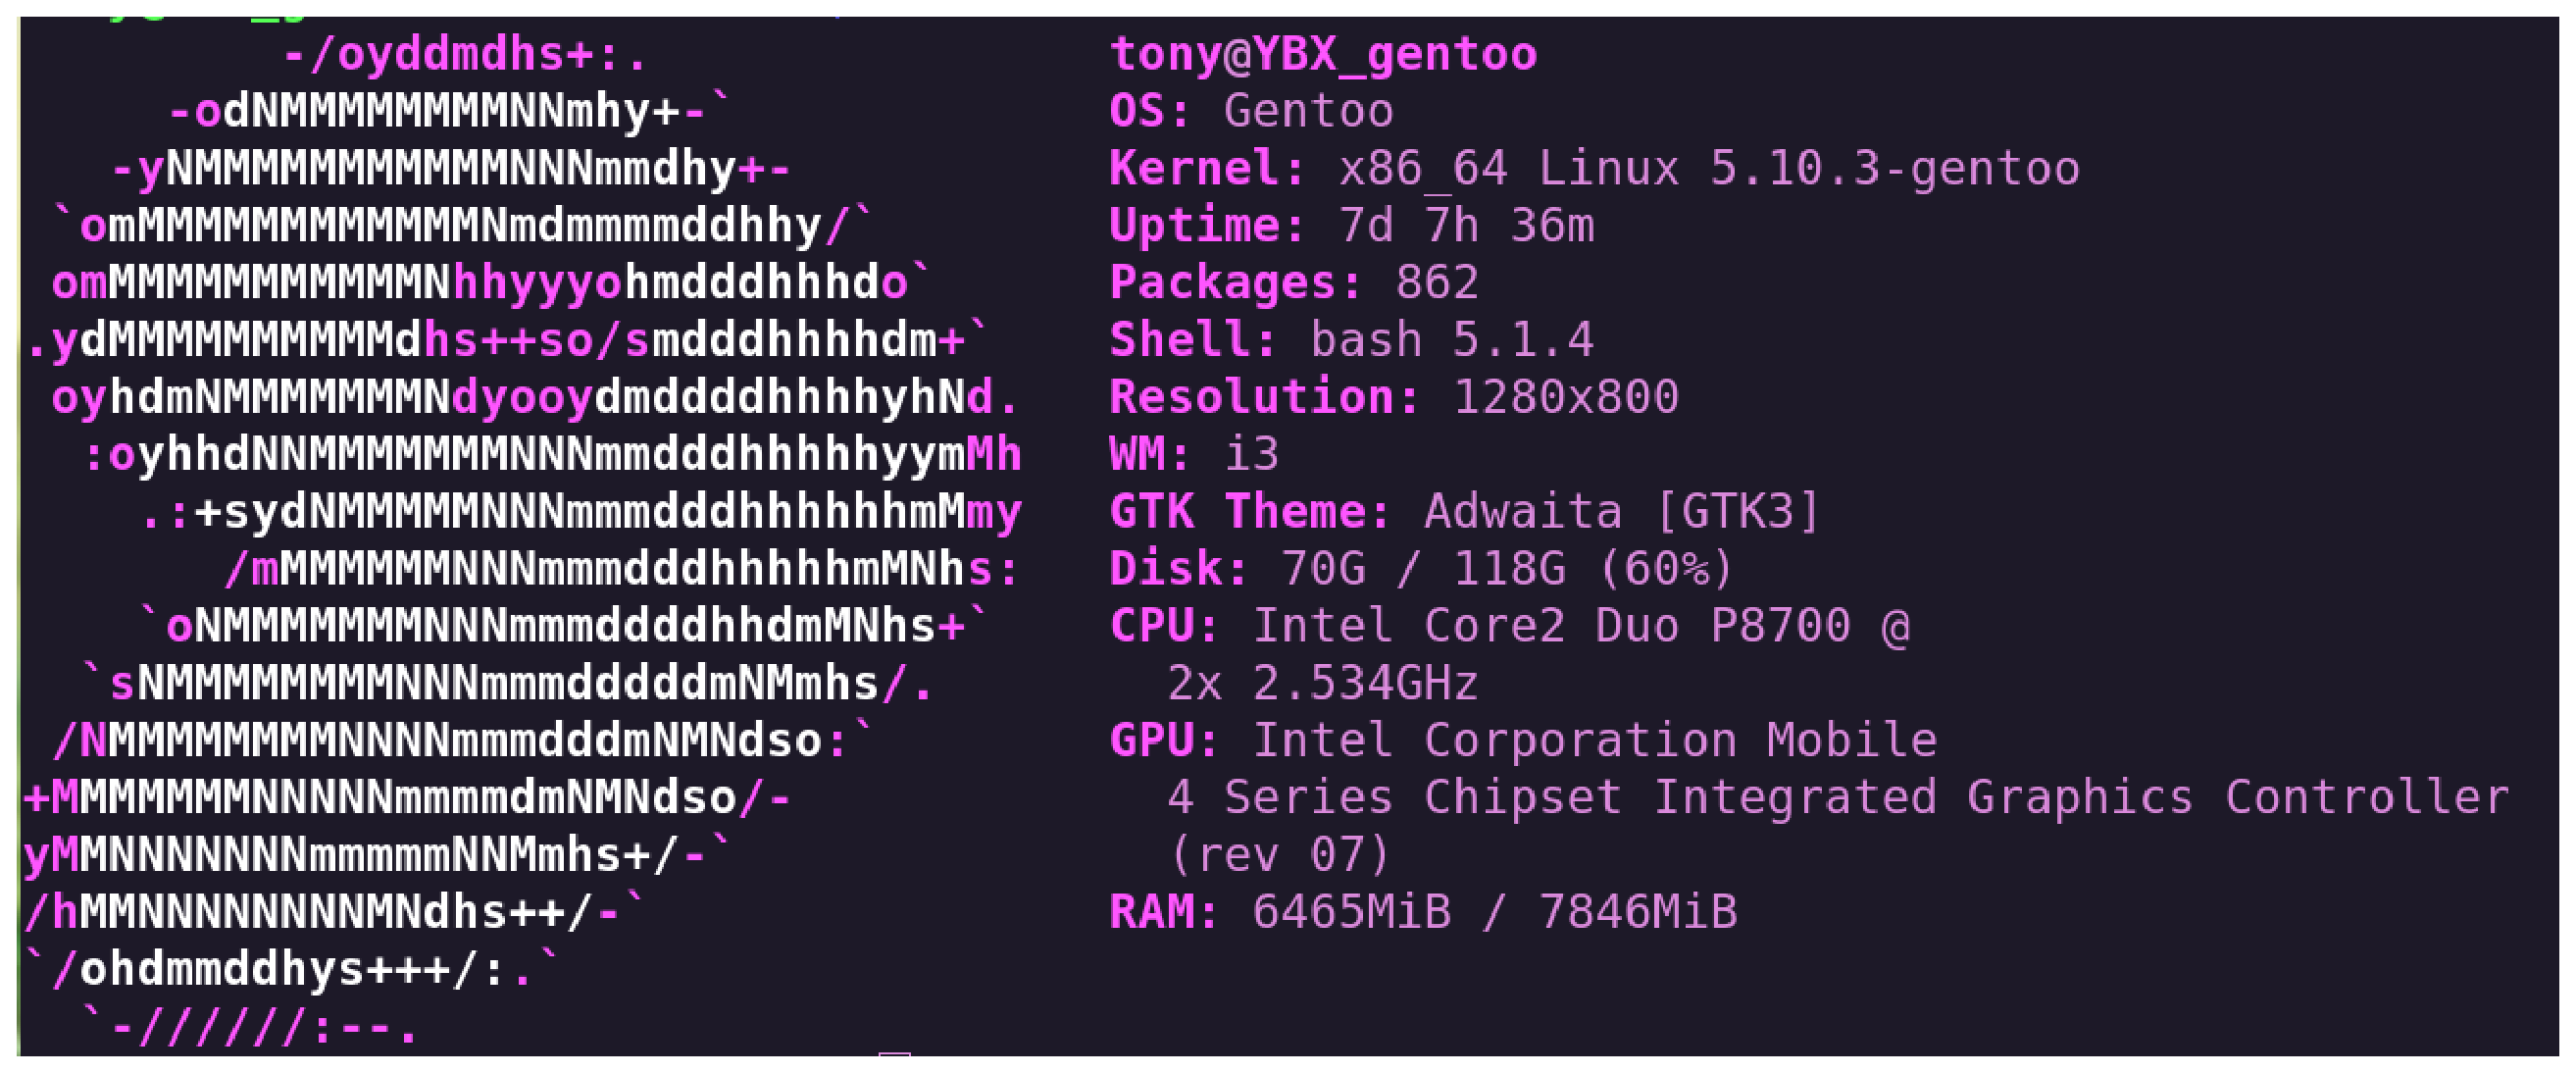
\includegraphics[width=0.6 \textwidth]{figs/gentoo_Logo.eps}
  \caption{实验操作系统}
  \label{fig:gentoo} %设置图形引用名称
\end{figure}

\subsection{Qemu搭建}
在 Gentoo 官方的 Wiki 手册中可以参考 \cite{GentooQemu}
\subsubsection{检测处理器是否支持虚拟化}
\begin{lstlisting}
\$ grep --color -E "vmx|svm" /proc/cpuinfo 
\end{lstlisting}
如果能显示出 图\ref{fig:vmx_svm} 说明处理器是支持虚拟化的

\begin{figure}[htbp]
  \centering %居中显示
  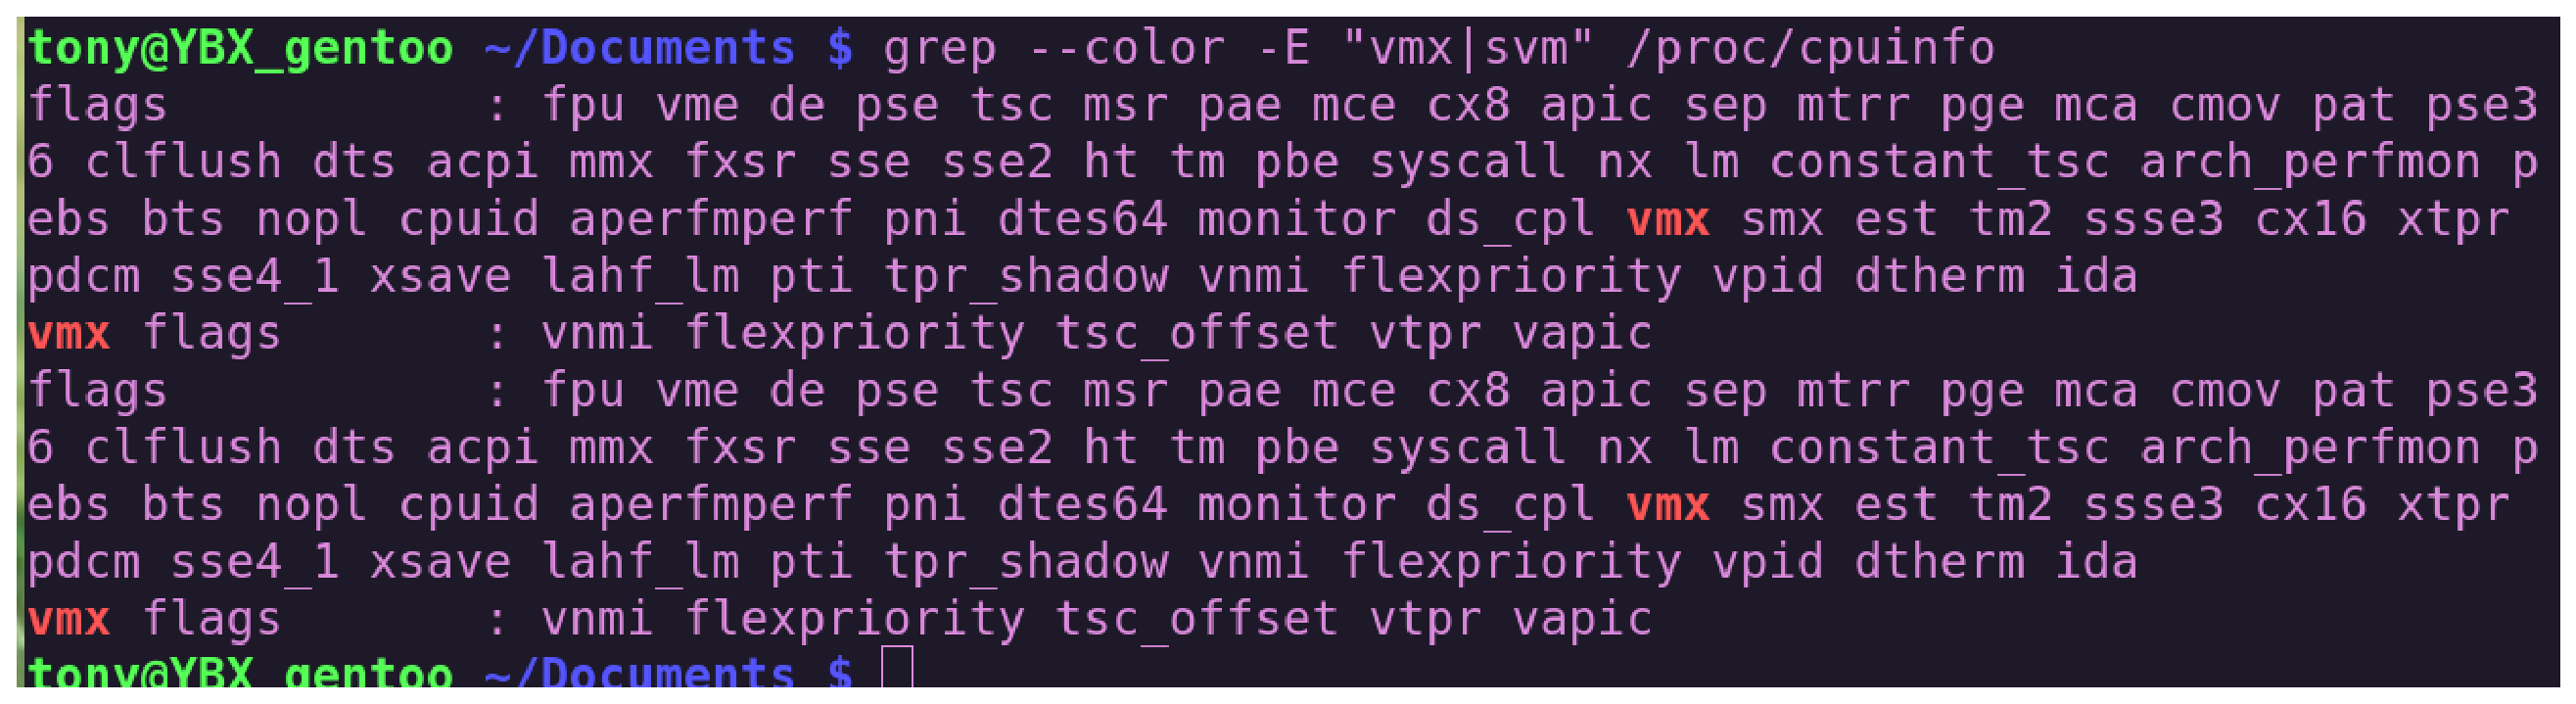
\includegraphics[width=0.6 \textwidth]{figs/vmx_svm.eps}
  \caption{是否支持虚拟化}
  \label{fig:vmx_svm} %设置图形引用名称
\end{figure}

\subsubsection{编译内核}
首先需要更改内核配置

\begin{lstlisting}
cd /usr/src/linux
make menuconfig 
\end{lstlisting}

然后根据以下步骤进行配置内核,使其支持KVM,其中 图\ref{fig:KVM_Intel} 是根据自己处理器来选择的,我的是Intel的处理器,如果使用AMD处理器的话,需要勾选另一个。

\begin{figure}[htbp]
  \centering %居中显示
  \includegraphics[width=0.9 \textwidth]{figs/Kernel/Step1.eps}
  \caption{Virtualization}
  \label{fig:Virtualization} %设置图形引用名称
\end{figure}

\begin{figure}[htbp]
  \centering %居中显示
  \includegraphics[width=0.9 \textwidth]{figs/Kernel/Step2.eps}
  \caption{Kernel-based Virtual Machine (KVM) support}
  \label{fig:Kernel-based} %设置图形引用名称
\end{figure}

\begin{figure}[htbp]
  \centering %居中显示
  \includegraphics[width=0.9 \textwidth]{figs/Kernel/Step3.eps}
  \caption{KVM for Intel processors support}
  \label{fig:KVM_Intel} %设置图形引用名称
\end{figure}

\subsubsection{修改USE Flags并安装}
\begin{lstlisting}
# vim /etc/portage/make.conf
QEMU_SOFTMMU_TARGETS="riscv32 risc64"
QEMU_USER_TARGETS="x86_64"

# vim /etc/portage/package.use
app-emulation/qemu qemu_softmmu_targets_arm qemu_softmmu_targets_x86_64 qemu_softmmu_targets_sparc
app-emulation/qemu qemu_user_targets_x86_64

% 进行安装
# emerge --ask app-emulation/qemu -y
\end{lstlisting}

\subsection{简便方法}
这个步骤是比较偷懒的方式,你可以直接下载网上已经提供编译好而且运行没问题的二进制包,直接运行,但是我下载了,就没运行成功,所以就没有截图演示。
\begin{lstlisting}
cd release
wget https://github.com/michaeljclark/busybear-linux/releases/download/v1.0/bbl.bz2
wget https://github.com/michaeljclark/busybear-linux/releases/download/v1.0/busybear.bin.bz2
bzip2 -d *.bz2
\end{lstlisting}

\subsection{安装GNU工具链}

\begin{lstlisting}
mkdir YBX-bishe
cd YBX-bishe/
# 拉取 gnu-toolchain
git clone --recursive https://github.com/riscv/riscv-gnu-toolchain

# 编译生成 RISC-V newlib & Linux toolchains
cd riscv-gnu-toolchain
./configure --prefix=/opt/riscv --enable-multilib
make newlib -j5
make linux -j5
export PATH=$PATH:/opt/riscv/bin
export RISCV=/opt/risc
$
\end{lstlisting}

\subsection{创建根文件系统}
\begin{lstlisting}
cd ..
git clone https://github.com/michaeljclark/busybear-linux.git
cd busybear-linux
make -j5
\end{lstlisting}

但是这没完,因为busybear会自动帮你下载好 busybox 但是需要自己进行解压和编译

\begin{lstlisting}
CROSS_COMPILE=riscv{{bits}}-unknown-linux-gnu- make menuconfig
CROSS_COMPILE=riscv{{bits}}-unknown-linux-gnu- make
\end{lstlisting}

下面咱们就要制做最小文件系统
\begin{lstlisting}
qemu-img create rootfs.img  1g
mkfs.ext4 rootfs.img
mkdir rootfs
sudo mount -o loop rootfs.img  rootfs
cd rootfs
sudo cp -r ../busyboxsource/_install/* .
sudo mkdir proc sys dev etc etc/init.d
cd etc/init.d/
sudo touch rcS
sudo vi rcS
#!/bin/sh
mount -t proc none /proc
mount -t sysfs none /sys
/sbin/mdev -s

sudo mod +x rcS
sudo umount rootfs
\end{lstlisting}

\subsection{构建Linux内核}
\begin{lstlisting}
git clone https://github.com/torvalds/linux
cd linux
git checkout v5.4
make ARCH=riscv CROSS_COMPILE=riscv64-unknown-linux-gnu- defconfig
make ARCH=riscv CROSS_COMPILE=riscv64-unknown-linux-gnu-
\end{lstlisting}

\subsection{制作BootLoader——BBL(Berkeley Boot Loader)}
\begin{lstlisting}
cd..
git clone https://github.com/riscv/riscv-pk.git
cd riscv-pk
mkdir build
cd build
../configure --enable-logo --host=riscv64-unknown-elf --with-payload=../../riscv-linux/vmlinux
make -j8
\end{lstlisting}

\subsection{运行}
\begin{lstlisting}
cd ..
mkdir Running
cd Running
\end{lstlisting}
创建KVM启动脚本
\begin{lstlisting}
vim open_kvm
#!/bin/sh
sudo /etc/init.d/libvirtd start
sudo virsh net-start default  #开启网络服务
\end{lstlisting}

创建KVM关闭脚本
\begin{lstlisting}
sudo virsh net-destory default
sudo /etc/init.d/libvirtd stop
\end{lstlisting}


创建网络启动脚本
\begin{lstlisting}
#!/bin/sh
brctl addif virbr0 $1
ifconfig $1 up
\end{lstlisting}

创建网络关闭脚本
\begin{lstlisting}
#!/bin/sh
ifconfig $1 down
brctl delif virbr0 $1
\end{lstlisting}

创建程序运行脚本
\begin{lstlisting}
#!/bin/sh
# QEMU 5.2以后.模拟器内部集成了OpenSBI
sudo qemu-system-riscv64 \
  -nographic -machine virt \
  -m 1024M \
  -kernel bbl \
  -kernel /home/tony/Documents/Risc-v/busybear-linux/build/linux-5.0/arch/riscv/boot/Image \
  -drive file=busybear.bin,format=raw,id=hd0 \
  -device virtio-blk-device,drive=hd0 \
  -device virtio-net-device,netdev=net0 \
  -netdev type=tap,script=./ifup.sh,downscript=./ifdown.sh,id=net0 \
  -append "root=/dev/vda ro console=ttyS0" 
\end{lstlisting}






\subsection{最终效果}
最终结果演示可以看 \cite{结果演示} 



